\chapter{Lists, Loops, and Conditionals}
% (Session 3 Bridge: Iris Classifier)

\section{Introduction}

\begin{tcolorbox}[title=Goal]
\textbf{Build} a simple rule-based Iris classifier using dictionaries, lists, loops, and conditionals, while keeping the logic sequential so it can be refactored into functions in Session 4.
\end{tcolorbox}

\begin{tcolorbox}[title=You will work in]
Use the following file for this session:
\begin{itemize}
    \item \texttt{session3/session3\_iris\_template.py} (main student file)
\end{itemize}
\textbf{How to run the file:} Always run this script from the project root using the terminal command: \\
\texttt{python3 session3/session3\_iris\_template.py} \\
\textbf{Do not edit other files.} We will reuse this file in later sessions.
\end{tcolorbox}

This session is a continuation of Session 2 (variables and basic data types) and is designed to bridge you into Session 4.
In Session 3, we intentionally keep the implementation \textbf{sequential} (no functions yet) so that Session 4 can refactor the exact same logic into reusable functions.

The task for Session 3 is to build a small rule-based classifier for the Iris dataset. You will use:
\begin{itemize}
    \item \textbf{lists} to store multiple samples,
    \item \textbf{dictionaries} to store a single sample with named keys,
    \item a \textbf{for loop} to process all samples,
    \item \textbf{if-else} conditionals to make predictions and evaluate them.
\end{itemize}

\begin{tcolorbox}[title=Hands-on file for this session]
Work only in the following file:
\begin{itemize}
    \item \texttt{session3/session3\_iris\_template.py}
\end{itemize}
\textbf{How to run the file:} Use \texttt{python3} in the integrated terminal or click the Run button in VS Code. \textbf{Do not edit other files.} We will reuse this file in later sessions.
\end{tcolorbox}

\section{What You Will Learn}
By the end of this tutorial, you will be able to:
\begin{enumerate}
    \item \textbf{Store structured data using dictionaries:} Represent one Iris flower sample using meaningful keys such as \texttt{petal\_length} and \texttt{species}.
    \item \textbf{Scale up using a list of dictionaries:} Combine many sample dictionaries into a single \texttt{dataset} list.
    \item \textbf{Automate repeated work using loops:} Use one loop to classify and evaluate every sample.
    \item \textbf{Use conditionals for decision making:} Apply a simple rule based on \texttt{petal\_length} and compute accuracy.
\end{enumerate}



\section{Continuity from Session 2 (Rule Variables)}
In Session 2 you introduced a simple rule with named variables. We keep those variables here \textbf{unchanged} because Session 4 expects the same naming and behavior.

The rule is:
\begin{quote}
If \texttt{petal\_length} is less than \texttt{threshold}, predict \texttt{setosa}; otherwise predict \texttt{not\_setosa}.
\end{quote}

Keep the following values exactly as they are in the session 3 template:

\begin{listing}[H]
\caption{Example Iris dataset variables}
\label{lst:iris_variables}
\begin{minted}[fontsize=\small, linenos, breaklines=true, frame=lines]{python}
sepal_length = 5.1
sepal_width = 3.5
petal_length = 1.4
petal_width = 0.2
species = "setosa"
\end{minted}
\end{listing}

\section{Python Lists}

A list in Python is a versatile data structure used to store ordered collections of items. Lists are ordered, mutable (you can change their contents). List can contain any type of data, such as numbers, strings, or even other lists (or dictionaries, as we'll see later).

Here's an example of a list containing numerical values, representing petal lengths:

\begin{minted}[fontsize=\small, linenos, breaklines=true, frame=lines, label=code:IrisPetalLengths]{python}
iris_petal_lengths = [
    1.4, 10.1, 1.7, 1.5,
    4.7, 4.5, 6.0, 5.1,
]
\end{minted}

\subsection{Accessing items in a list:} Python lists are indexed starting from zero. You access individual items using square brackets:
\begin{minted}[fontsize=\small, linenos, breaklines=true]{python}
first_petal_length = iris_petal_lengths[0]   # 1.4
second_petal_length = iris_petal_lengths[1]  # 10.1
\end{minted}

\subsection{Changing list items:} 
Lists are mutable, meaning you can modify their values. For example, to change the first petal length:
\begin{minted}[fontsize=\small, linenos, breaklines=true]{python}
iris_petal_lengths[0] = 1.5  # Changes the first petal length to 1.5
\end{minted}

\subsection{Adding items to a list:} 
You can append new values to the list easily. For example, to add a new petal length,
\begin{minted}[fontsize=\small, linenos, breaklines=true]{python}
iris_petal_lengths.append(4.0)  # Adds a new value at the end
\end{minted}

% Now you have a basic understanding of Python lists. We will use lists to hold multiple flower dictionaries.

\section{Concept: Dictionaries (One Iris Sample)}
\label{sec:dictionaries}

\subsubsection{Introduction to Dictionaries}
\label{sec:ses3_dictionaries}

Dictionaries are a fundamental data structure in Python used for storing collections of \textbf{key-value pairs}. Unlike lists, which are ordered sequences accessed by numerical index, dictionaries are unordered collections where you access data using \textbf{keys}. Think of a real-world dictionary: you look up a word (the key) to find its definition (the value).

Dictionaries are incredibly useful when you need to associate pieces of information with specific labels or identifiers, making your code more readable and maintainable.

In our previous sessions, we've seen how to store individual pieces of information using separate variables. While this works for a small amount of data, it quickly becomes cumbersome when dealing with many flowers or features.

Using a dictionary, we can group related pieces of information under meaningful names. For example, we can convert the code variables (as in block  \ref{lst:iris_variables}) into a single dictionary that represents one flower sample as shown in block \ref{lst: iris_dictionary}.

%  Below is an illustrative example of what a dictionary looks like (note the curly braces \texttt{\{} and \texttt{\}}). You do not need to type this verbatim yet:

\begin{listing}[H]
\caption{Example Iris dataset variables}
\label{lst: iris_dictionary}

\begin{minted}[fontsize=\small, linenos, breaklines=true, frame=lines]{python}
sample = {
    "id": "flower1",
    "sepal_length": 5.1,
    "sepal_width": 3.5,
    "petal_length": 1.4,
    "petal_width": 0.2,
    "species": "setosa"
}
\end{minted}
\end{listing}

In this example, "id", "sepal\_length", "sepal\_width", "petal\_length", "petal\_width", and "species" are keys, and their corresponding values are the data associated with each key. Notice that values can be of different types, including strings, nested dictionaries, and lists.

\begin{lectureronly}
Ask student, about which is string, which is number, and which is a label. This is a good opportunity to reinforce the concept of data types in the context of dictionaries.
\end{lectureronly}

\subsection{Creating Dictionaries}
\label{subsubsec:creating_dicts}
There are several ways to define a dictionary in Python. Let's explore three common methods:

\begin{itemize}
\item \textbf{Literal syntax (\texttt{\{\}}):} This is the most direct and common way to create dictionaries.
\item \textbf{Using \texttt{dict([])} with tuples:} This method involves passing a list of tuples to the \texttt{dict()} constructor.
\item \textbf{Using \texttt{dict()} with keyword arguments:} This approach uses the \texttt{dict()} constructor and assigns key-value pairs using keyword-like syntax.
\end{itemize}

\paragraph{Literal Syntax \texttt{\{\}}}
This is the most straightforward way to create a dictionary. You enclose key-value pairs within curly braces \texttt{\{\}}. Each key-value pair is separated by a colon \texttt{:}, and pairs are separated by commas \texttt{,}:

\begin{minted}[fontsize=\small, linenos, breaklines=true, frame=lines]{python}
flower_parts = {
    "id": "flower1",
    "sepal_length": 5.1,
    "sepal_width": 3.5,
    "petal_length": 1.4,
    "petal_width": 0.2,
    "species": "setosa"
}
\end{minted}

\paragraph{\texttt{dict([])} with Tuples}
You can also create a dictionary by passing a list of tuples to the \texttt{dict()} constructor:

\begin{minted}[fontsize=\small, linenos, breaklines=true, frame=lines]{python}
flower_parts = dict([
    ("id", "flower1"),
    ("sepal_length", 5.1),
    ("sepal_width", 3.5),
    ("petal_length", 1.4),
    ("petal_width", 0.2),
    ("species", "setosa")
])
\end{minted}
This is useful when your data is already structured as key-value pairs in tuples.

\paragraph{\texttt{dict()} with Keyword Arguments}
The \texttt{dict()} function can also be used with keyword arguments. This is often more readable when creating dictionaries with string keys:

\begin{minted}[fontsize=\small, linenos, breaklines=true, frame=lines]{python}
flower_sample1 = dict(
    id="flower1",
    sepal_length=5.1,
    sepal_width=3.5,
    petal_length=1.4,
    petal_width=0.2,
    species="setosa"
)
\end{minted}

Regardless of the method you choose, the variable now holds a dictionary representing a flower's measurements.

\begin{tcolorbox}[title=Canonical Keys are Important!]
Before you start the task, it is critical to use these exact keys: \texttt{id}, \texttt{sepal\_length}, \texttt{sepal\_width}, \texttt{petal\_length}, \texttt{petal\_width}, and \texttt{species}. Later code (in Session 4 and beyond) relies on these canonical names for dictionary lookups. If you misspell them, the code will fail to find the values!
\end{tcolorbox}





\subsection{Your Task: Replacing sequential variable declaration with dict}


\noindent
\begin{tcolorbox}[title=Task 1: Create A dictionary for second flower]
... but use the same values from Session 2 (the setosa image) and remove the \texttt{\_2} suffix from the keys.
\end{tcolorbox}


Open the file \texttt{session3/session3\_iris\_template.py}. 
We will now convert the variables you created in Session 2 into a dictionary format. 
For the second flower (\texttt{flower2}), remove the \texttt{\_2} suffix from the keys (e.g., use \texttt{sepal\_length} instead of \texttt{sepal\_length\_2}), but keep the numerical values from the Session 2 setosa image.

\begin{figure}[H]
    \centering
    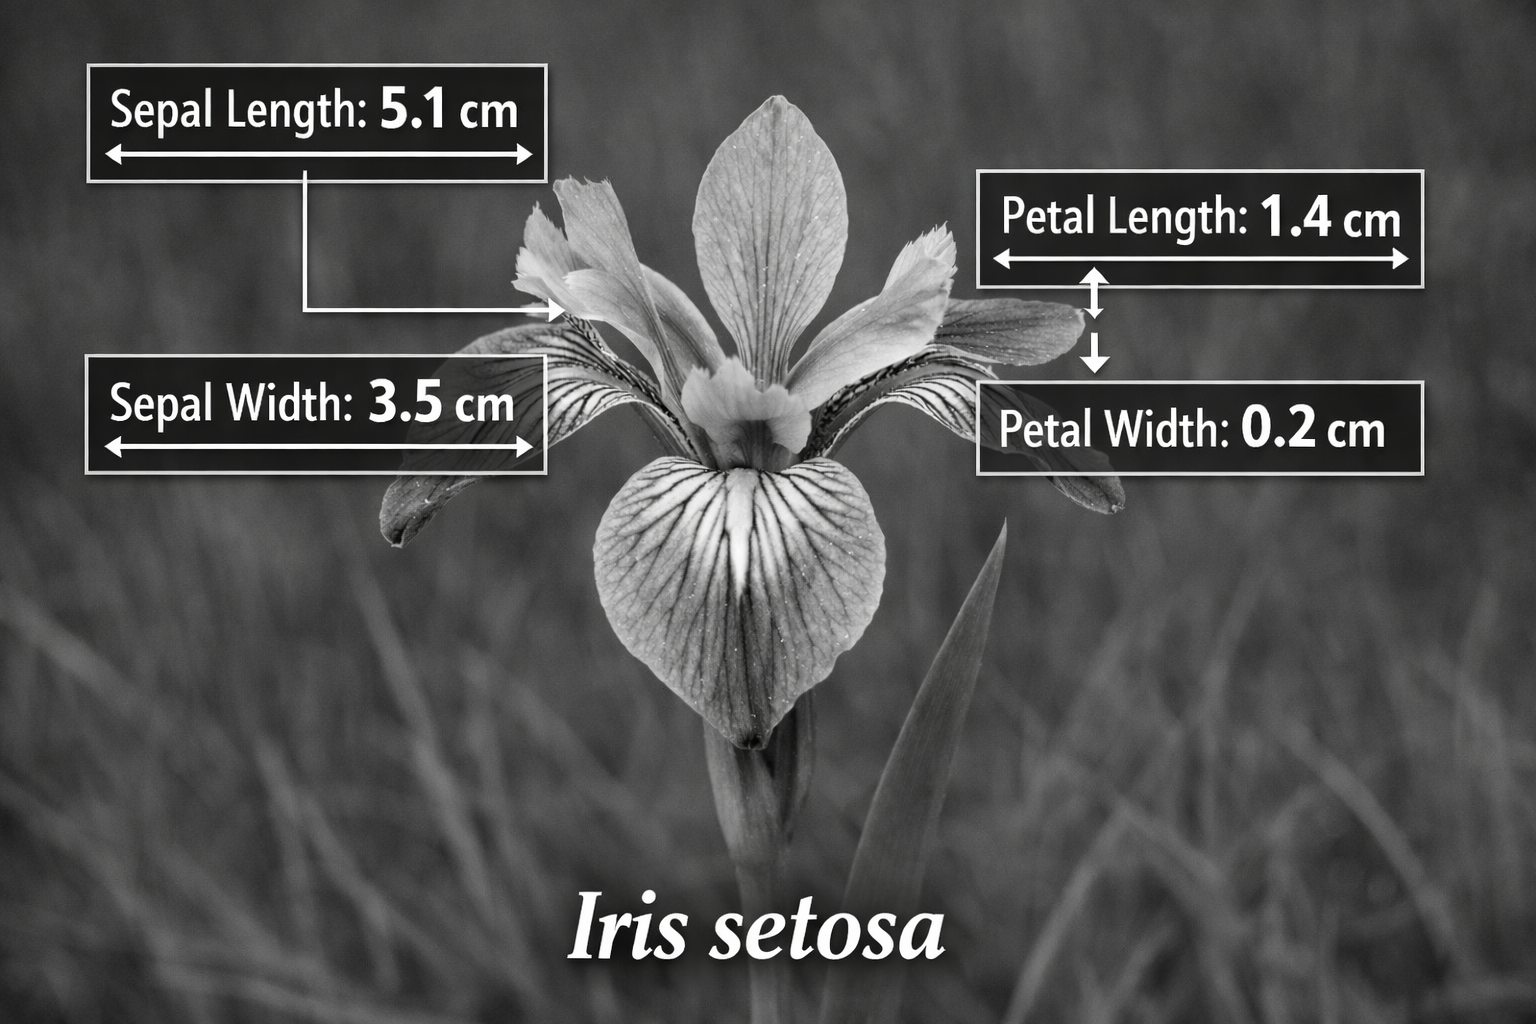
\includegraphics[width=0.5\textwidth]{session2/image/iris_setosa.png}
    \caption{Iris setosa flower measurements (recap from Session 2).}
\end{figure}

\begin{tcolorbox}[title=Hint]
Use the same measurements from Session 2 but without the \texttt{\_2} suffix when building the dictionary for \texttt{flower2}.
\end{tcolorbox}

\begin{tcolorbox}[title=Checkpoint]
You should have two dictionaries defined: \texttt{flower1} and \texttt{flower2}, using literal syntax \texttt{\{\}}.
\end{tcolorbox}


\begin{tcolorbox}[title=Common Mistakes]
Make sure you didn't forget commas at the end of each key-value pair, and ensure the keys have quotes around them (e.g., \texttt{"sepal\_length"}).
\end{tcolorbox}

\subsection{Accessing Data from Dictionaries}
You access values in a dictionary using their corresponding \textbf{keys} within square brackets \texttt{[]}.

\begin{minted}[fontsize=\small, linenos, breaklines=true, frame=lines]{python}
print(flower_sample1['id']) # Print the id of the flower
\end{minted}

\begin{lectureronly}
    \textbf{Solution:}
    The student should create a dictionary for the second flower using the values from the image:
    
    \begin{minted}[fontsize=\small, linenos]{python}
flower2 = {
    "id": "flower2",
    "sepal_length": 4.9,
    "sepal_width": 3.0,
    "petal_length": 1.4,
    "petal_width": 0.2,
    "species": "setosa"
}
    \end{minted}
\end{lectureronly}

\section{List of Dictionaries}
\label{sec:ses3_list_of_dicts}

\noindent
\begin{tcolorbox}[title=Task 2: Create list of dictionaries]
Combine your two flower dictionaries into a list called \texttt{dataset}.
\end{tcolorbox}

One Iris sample is useful, but the real task is to process \textbf{many} samples.
We therefore store multiple dictionaries inside a list called \texttt{dataset}.

Start from this pattern (your template already contains a filled example for flower 1, but you'll combine them):
\begin{minted}[fontsize=\small, linenos, breaklines=true, frame=lines]{python}
dataset = [flower1, flower2]
\end{minted}

\begin{tcolorbox}[title=Checkpoint]
Ensure \texttt{dataset} is a list containing your two dictionary variables.
\end{tcolorbox}

\section{For Loop}

A \textbf{for loop} lets you run the \emph{same} block of code multiple times without copying and pasting it. It is especially useful when you want to process \textbf{each item in a sequence} (for example: a list of numbers, a list of strings, or a dataset).

\subsection{The Core Idea: ``Do this for each item''}
Think of a for loop as reading a list one element at a time:
\begin{quote}
``For each item in this collection, run these instructions.''
\end{quote}

Most for loops involve a \textbf{loop variable} (a temporary name you choose) that takes on a new value each iteration.

For example, conceptually iterating from $1$ to $n$ looks like:
\[
\text{for } i = 1 \text{ to } n \text{ do: execute the loop body.}
\]
Here, $i$ is the loop variable and it changes as the loop runs.

\subsection{What Parts Make Up a Loop?}
In many languages, a for loop can be described using four pieces:
\begin{itemize}
  \item \textbf{Initialization:} where the loop starts (e.g., $i=1$).
  \item \textbf{Condition:} when the loop should stop (e.g., keep going while $i \le n$).
  \item \textbf{Update:} how the loop variable changes each time (e.g., $i \leftarrow i+1$).
  \item \textbf{Body:} the code that repeats each iteration.
\end{itemize}

\noindent
In Python, you most often write for loops in the simpler ``for each item in this sequence'' style, which avoids manually writing the condition and update step.

\subsection{Looping Over the Dataset}
\label{sec:ses3_loop}


\begin{tcolorbox}[title=Task 3: Create a for loop to process the dataset]
Write a for loop that processes each sample in the \texttt{dataset} list. Inside the loop, print the sample's \texttt{id}, \texttt{petal\_length}, and \texttt{species}.
\end{tcolorbox}

When you have a dataset stored as a \textbf{list of dictionaries}, one of the cleanest ways to process every sample is a \texttt{for} loop. The loop below assigns each dictionary to the variable \texttt{sample}, one at a time:

\begin{minted}[fontsize=\small, linenos, breaklines=true, frame=lines]{python}
for sample in dataset:
    print(sample["id"], sample["petal_length"], sample["species"])
\end{minted}

\subsubsection{How to Read This Code}
\begin{itemize}
  \item \texttt{dataset} is the full collection (a list).
  \item \texttt{sample} is one element from that list (a dictionary).
  \item On each iteration, \texttt{sample} refers to a \emph{different} dictionary.
\end{itemize}

\begin{tcolorbox}[title=Good Practice]
The \texttt{print} step is a good beginner-friendly debugging habit:
\begin{itemize}
  \item It confirms the keys (like \texttt{"id"} and \texttt{"petal\_length"}) actually exist.
  \item It lets you check that values look reasonable before adding more logic.
\end{itemize}

Use debug line by line to understand what is happening inside the for loop
\end{tcolorbox}





\noindent
Once you trust the data shape and values, you can replace the \texttt{print} line with classification or processing code.


\section{Conditionals}
A \textbf{conditional} lets your program \textbf{make a decision} based on data. In many application, the most common form is an \textbf{if--else} statement:

\subsection{Conditionals for Classification}
Next, we will introduce 3 conditional statements within the loop.Basiclly, this include the task 4, task 5, and task 6.

\label{sec:ses3_conditionals}




\begin{itemize}
  \item if a condition is \texttt{True}, run the indented ``if'' block;
  \item otherwise, run the indented ``else'' block.
\end{itemize}

\subsubsection{Using a Rule to Predict a Label}
In our classifier, the decision rule compares \textbf{one feature value} to a \textbf{threshold}. The variable \texttt{feature\_name} tells us which feature to look up in the current \texttt{sample} dictionary:

\begin{tcolorbox}[title=Task 4: Use an if-else statement to classify each sample based on the threshold rule]

Use the if else statement, so that, if the chosen feature value is less than the threshold, set \texttt{y\_pred} to \texttt{positive\_label}; otherwise, set it to \texttt{negative\_label}.
\end{tcolorbox}

Specifically, we will use the following code pattern to classify each sample based on the rule defined in Session 2. This code should be placed inside the for loop that processes each sample:
\begin{minted}[fontsize=\small, linenos, breaklines=true, frame=lines]{python}
    if sample[FEATURE_NAME] < THRESHOLD:
        y_pred = POSITIVE_LABEL
    else:
        y_pred = NEGATIVE_LABEL
\end{minted}

We can read the code as follow
\begin{itemize}
  \item \texttt{sample[FEATURE\_NAME]} retrieves the feature value (e.g., \texttt{sample["petal\_length"]}).
  \item \texttt{< THRESHOLD} checks whether that value is below the cutoff.
  \item \texttt{y\_pred} stores the predicted label for this sample.
\end{itemize}

\begin{tcolorbox}[title=Common Mistakes]

\begin{itemize}
  \item \textbf{Indentation matters:} the indented lines belong to the \texttt{if} or \texttt{else} block.
  \item \textbf{Exactly one branch runs:} either the \texttt{if} block or the \texttt{else} block, never both.
  \item If you want ``less than or equal,'' use \texttt{<=} instead of \texttt{<}.
\end{itemize}
\end{tcolorbox}








% \subsection{Task 1: Initialize Metrics and Predictions List}
% Before the loop, initialize counters and a list for predictions:
% \begin{minted}[fontsize=\small, linenos, breaklines=true, frame=lines]{python}
% correct = 0
% wrong = 0
% total = 0
% y_pred_list = []
% \end{minted}

\subsubsection{Assign Classification Rule}
\label{sec:ses3_required_bridge}
Inside the loop, compute \texttt{y\_pred} using the Session 2 rule. Do \textbf{not} define any functions yet.

\subsection{Task 5: Derive the True Label (\texttt{y\_true})}
The next placeholder in the template asks you to convert the stored species into the two-label format used by the rule. Keep this code inside the same \texttt{for} loop:
\begin{minted}[fontsize=\small, linenos, breaklines=true, frame=lines]{python}
    if sample[LABEL_KEY] == POSITIVE_LABEL:
        y_true = POSITIVE_LABEL
    else:
        y_true = NEGATIVE_LABEL
\end{minted}

This step is important because we want the \texttt{true} label and the \texttt{predicted} label to use the same naming scheme:
\begin{itemize}
    \item if the flower really is \texttt{"setosa"}, then \texttt{y\_true} becomes \texttt{POSITIVE\_LABEL},
    \item otherwise, \texttt{y\_true} becomes \texttt{NEGATIVE\_LABEL}.
\end{itemize}

\begin{tcolorbox}[title=Task 5:. Derive true label (y\_true) from the dataset sample]
Read the real species from \texttt{sample[LABEL\_KEY]} and store the converted result in \texttt{y\_true}.
\end{tcolorbox}

\subsection{Task 6: Update Correct or Wrong Counter}
Once both \texttt{y\_pred} and \texttt{y\_true} exist, compare them. If they match, increase \texttt{correct}; otherwise increase \texttt{wrong}.
\begin{minted}[fontsize=\small, linenos, breaklines=true, frame=lines]{python}
    if y_pred == y_true:
        correct += 1
    else:
        wrong += 1
\end{minted}

\begin{tcolorbox}[title=Task 6: Update correct or wrong counter]
Only one counter should increase for each sample: either \texttt{correct} or \texttt{wrong}.
\end{tcolorbox}

\subsection{Task 7: Always Increment \texttt{total}}
\begin{tcolorbox}[title=Task 7: ALWAYS increment total for every sample processed]
Increase \texttt{total} once for every sample that goes through the loop.
\end{tcolorbox}

Every sample that reaches the loop has been processed, so \texttt{total} must increase every time, regardless of whether the prediction was right or wrong:
\begin{minted}[fontsize=\small, linenos, breaklines=true, frame=lines]{python}
    total += 1
\end{minted}

\subsection{Task 8: Append the Prediction to \texttt{y\_pred\_list}}
\begin{tcolorbox}[title=Task 8: Append the prediction to our list]
Store the current \texttt{y\_pred} by appending it to \texttt{y\_pred\_list}.
\end{tcolorbox}

The template also asks you to keep a record of all predictions. Add the current prediction to the list:
\begin{minted}[fontsize=\small, linenos, breaklines=true, frame=lines]{python}
    y_pred_list.append(y_pred)
\end{minted}

\noindent
After Tasks 5 to 8, your loop is now doing four jobs:
\begin{itemize}
    \item converting the true species into \texttt{y\_true},
    \item updating the correct/wrong counters,
    \item increasing the total number of processed samples,
    \item storing every prediction in \texttt{y\_pred\_list}.
\end{itemize}

\begin{tcolorbox}[title=Checkpoint]
Your loop should be processing each sample. \textbf{Self-check:} Does \texttt{total} increase for every sample processed? Even if the prediction is wrong, \texttt{total} must increase by 1.
\end{tcolorbox}
\begin{tcolorbox}[title=Common Mistakes]
Forgetting to increment \texttt{total} inside the loop, or accidentally only incrementing it if the prediction was correct.
\end{tcolorbox}

\subsection{Task 9: Print Per-Sample Trace Lines}
\begin{tcolorbox}[title=Task 9: Print per-sample trace exactly as required]
Uncomment the print block so each processed sample shows its id, true label, predicted label, and petal length.
\end{tcolorbox}

The template leaves the print block commented out. Uncomment it so you can see exactly what happened for each flower:
\begin{minted}[fontsize=\small, linenos, breaklines=true, frame=lines]{python}
print(
    f"id={sample['id']} | true={y_true} | pred={y_pred} | "
    f"petal_length={sample['petal_length']}"
)
\end{minted}

\noindent
This trace line is useful because it shows:
\begin{itemize}
    \item which flower is being processed,
    \item the true label,
    \item the predicted label,
    \item the feature value used by the rule.
\end{itemize}

\subsection{Task 10: Final Summary (After the Loop)}
\begin{tcolorbox}[title=Task 10: Compute and print final metrics]
After the loop ends, compute \texttt{accuracy} and print the summary lines already present in the template.
\end{tcolorbox}

Task 10 happens \textbf{after} the loop finishes. First compute the accuracy:
\begin{minted}[fontsize=\small, linenos, breaklines=true, frame=lines]{python}
accuracy = (correct / total) * 100 if total > 0 else 0.0
\end{minted}

Then uncomment the summary print statements already provided in the template:
\begin{minted}[fontsize=\small, linenos, breaklines=true, frame=lines]{python}
print("\n=== session 3 Summary ===")
print("Correct:", correct)
print("Wrong:", wrong)
print("Total:", total)
print("Accuracy (%):", round(accuracy, 2))
print("All predictions:", y_pred_list)
\end{minted}

\begin{tcolorbox}[title=Checkpoint and this is what is expected in ITEL]
You should see output similar to this at the end: \\
\texttt{Correct: 2} \\
\texttt{Wrong: 0} \\
\texttt{Total: 2} \\
\texttt{Accuracy (\%): 100.0} \\
\texttt{All predictions: ['setosa', 'setosa']}
\end{tcolorbox}

\section{Expected Output When Submitting in Itel}

In the terminal, you should see the following output when running the program:
\begin{minted}[fontsize=\small, linenos, breaklines=true, frame=lines]{python}
=== Start session 3 Prediction Loop ===
flower1 1.4 setosa
id=flower1 | true=setosa | pred=setosa | petal_length=1.4
flower2 1.4 setosa
id=flower2 | true=setosa | pred=setosa | petal_length=1.4

=== session 3 Summary ===
Correct: 2
Wrong: 0
Total: 2
Accuracy (%): 100.0
All predictions: ['setosa', 'setosa']
\end{minted}

\section{Summary \& Review}
\begin{itemize}
    \item \textbf{Dictionaries:} You learned to store one object's features using named keys.
    \item \textbf{Lists:} You used lists to hold multiple dictionary items.
    \item \textbf{Loops:} You iterated over the dataset using a \texttt{for} loop.
    \item \textbf{Conditionals:} You used \texttt{if}/\texttt{else} to classify samples.
    \item \textbf{Metrics:} You tracked accuracy by counting correct predictions over total samples.
\end{itemize}

\textbf{Reflection Questions:}
\begin{enumerate}
    \item Why is a list of dictionaries better than having many individual variables (like \texttt{sepal\_length\_2}, \texttt{sepal\_length\_3})?
    \item What happens to your dictionary lookups if you misspell a key?
\end{enumerate}

\textbf{Micro-Exercise:} Add a third sample to your \texttt{dataset} (e.g., make up a flower with \texttt{petal\_length: 4.5} and \texttt{species: "versicolor"}). Run the script again and observe how the loop, trace lines, and accuracy automatically update!
